{
\begin{table}[h!]
    \centering
    \begin{tabular}{|p{3cm}|p{15cm}|} 
        \hline
        \rowcolor{TableBgRowColor}        
        \cellcolor{HighVulnColor} \textbf{CWE} & 
        \textbf{\href{https://cwe.mitre.org/data/definitions/522.html}{CWE-522} } \\
        \hline
        \rowcolor{TableBgRowIntemediaColor}
        \cellcolor{HighVulnColor} \textbf{Puntuación CVSS 3.1} & 
        \textbf{9.5} \\
        \hline
        \rowcolor{TableBgRowColor}
        \cellcolor{HighVulnColor} \textbf{Impacto} & 
        \textbf{9.5 (AV:N/AC:L/PR:N/UI:N/S:U/C:H/I:H/A:H)} \\
        \hline
        \rowcolor{TableBgRowIntemediaColor}        
        \cellcolor{HighVulnColor} \textbf{Descripción (Incl. Causa Raíz)} & 
        \textbf{Respondiendo al tráfico de red LLMNR/NBT-NS} \\
        \hline        
        \rowcolor{TableBgRowColor}        
        \cellcolor{HighVulnColor} \textbf{Impacto de Seguridad} & 
        \textbf{Los adversarios pueden suplantar una autoridad} \\
        \hline
        \rowcolor{TableBgRowIntemediaColor}        
        \cellcolor{HighVulnColor} \textbf{Dominio Afectado} & 
        \textbf{INLANEFREIGHT.LOCAL} \\
        \hline
        \rowcolor{TableBgRowColor}        
        \cellcolor{HighVulnColor} \textbf{Remediación} & 
        \textbf{
Deshabilitar LLMNR y NetBIOS en la configuración de seguridad del equipo local o mediante políticas de grupo si no son necesarios en el entorno. 
Usar software de seguridad basado en el host para bloquear el tráfico LLMNR/NetBIOS. Habilitar la firma SMB puede detener los ataques de retransmisión NTLMv2. 
Los sistemas de detección y prevención de intrusiones que identifiquen patrones de tráfico indicativos de actividad MiTM pueden mitigar la actividad a nivel de red. 
La segmentación de red puede usarse para aislar componentes de infraestructura que no requieran acceso amplio a la red. Esto puede mitigar, o al menos aliviar, el alcance de la actividad MiTM. 
        } \\
        \hline
        \rowcolor{TableBgRowIntemediaColor}        
        \cellcolor{HighVulnColor} \textbf{Referencias Externas} & 
        \textbf{\url{https://attack.mitre.org/techniques/T1557/001/}} \\
        \hline
    \end{tabular}
\end{table}

% Repetimos para MediumVulnColor
\begin{table}[h!]
    \centering
    \begin{tabular}{|p{3cm}|p{15cm}|} 
        \hline
        \rowcolor{TableBgRowColor}        
        \cellcolor{MediumVulnColor} \textbf{CWE} & 
        \textbf{\href{https://cwe.mitre.org/data/definitions/522.html}{CWE-522} } \\
        \hline
        \rowcolor{TableBgRowIntemediaColor}
        \cellcolor{MediumVulnColor} \textbf{Puntuación CVSS 3.1} & 
        \textbf{9.5} \\
        \hline
        \rowcolor{TableBgRowColor}
        \cellcolor{MediumVulnColor} \textbf{Impacto} & 
        \textbf{9.5 (AV:N/AC:L/PR:N/UI:N/S:U/C:H/I:H/A:H)} \\
        \hline
        \rowcolor{TableBgRowIntemediaColor}        
        \cellcolor{MediumVulnColor} \textbf{Descripción (Incl. Causa Raíz)} & 
        \textbf{Respondiendo al tráfico de red LLMNR/NBT-NS} \\
        \hline        
        \rowcolor{TableBgRowColor}        
        \cellcolor{MediumVulnColor} \textbf{Impacto de Seguridad} & 
        \textbf{Los adversarios pueden suplantar una autoridad} \\
        \hline
        \rowcolor{TableBgRowIntemediaColor}        
        \cellcolor{MediumVulnColor} \textbf{Dominio Afectado} & 
        \textbf{INLANEFREIGHT.LOCAL} \\
        \hline
        \rowcolor{TableBgRowColor}        
        \cellcolor{MediumVulnColor} \textbf{Remediación} & 
        \textbf{(Texto igual que el anterior)} \\
        \hline
        \rowcolor{TableBgRowIntemediaColor}        
        \cellcolor{MediumVulnColor} \textbf{Referencias Externas} & 
        \textbf{\url{https://attack.mitre.org/techniques/T1557/001/}} \\
        \hline
    \end{tabular}
\end{table}

Evidencia de los Hallazgos: \\
\textbf{Ejecutando la herramienta Responder para intentar obtener los hashes de contraseñas de cuentas de usuario.} \\

\begin{figure}[H]
    \centering
    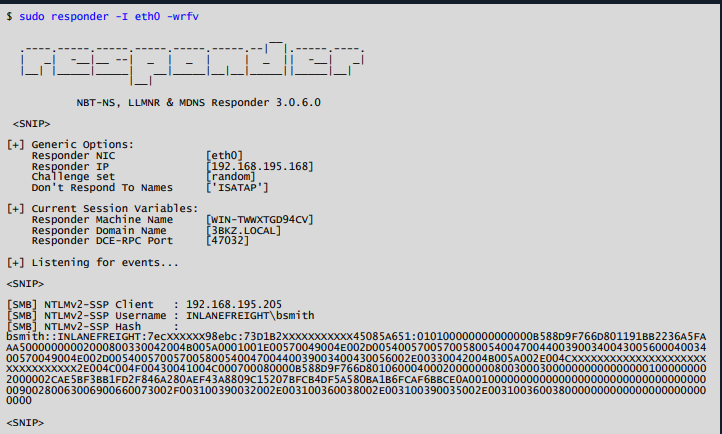
\includegraphics[width=1\linewidth]{initial//evidenceimages/responder.png}
    \caption{Introducir leyenda aquí}
    \label{fig:enter-label}
\end{figure}

\textbf{Descifrado exitoso de un hash de contraseña con Hashcat para revelar el valor en texto claro.}

% Repetimos para LowVulnColor
% Similar estructura que las anteriores tablas.
}
